\documentclass{article}


\usepackage[preprint]{neurips_2026}


\usepackage[utf8]{inputenc} % allow utf-8 input
\usepackage[T1]{fontenc}    % use 8-bit T1 fonts
\usepackage{hyperref}       % hyperlinks
\usepackage{url}            % simple URL typesetting
\usepackage{booktabs}       % professional-quality tables
\usepackage{amsfonts}       % blackboard math symbols
\usepackage{amsmath}        % math
\usepackage{nicefrac}       % compact symbols for 1/2, etc.
\usepackage{microtype}      % microtypography
\usepackage{xcolor}         % colors
\usepackage{graphicx}       % figures
\usepackage{multirow}       % table cells

\graphicspath{{figures/}}


\title{The Alignment Tax on Humor is a Safety--Fine-Tuning Tax, Not an RLHF Tax}


\author{%
  Karthik Bhattaram \\
  Humor Alignment Tax Project \\
  \texttt{saberlight35@gmail.com} \\
}


\begin{document}


\maketitle


\begin{abstract}
A common worry about language-model safety training is that it imposes an \emph{alignment tax} on creativity: by steering models toward safe, predictable text it may flatten the statistical properties that make outputs surprising, clever, and funny. We test this directly on humor using Llama~3.2~1B across three alignment tiers (base, RLHF-instruct, instruct~+~LoRA safety fine-tune), three judge-independent distributional metrics (punchline surprisal, pre-punchline entropy, setup--punchline embedding distance), an LLM-as-judge rubric, and linear probes. We find four things. (i)~The humor tax is \emph{non-monotonic}: RLHF does not tax humor---instruct jokes are rated as funny as a human corpus ($6.77$ vs.\ $6.71$/$10$)---whereas the safety fine-tune collapses humor ($\to 3.24$), driven by a $74\%$ refusal rate on benign joke prompts. (ii)~Alignment \emph{widens} rather than compresses all three metrics at every stage (entropy $+0.44$ instruct$\to$safety), the opposite of the compression hypothesis, and this replicates cross-lingually on Chinese Oogiri and Ruozhiba humor ($d$ $0.43$--$0.83$). (iii)~The classic inverted-U between distributional ``surprise'' and rated humor is not supported ($R^2\le0.09$), and raising temperature monotonically \emph{lowers} humor. (iv)~The tax is \emph{asymmetric}: fine-tuning for humor does not erode AdvBench/HarmBench safety (refusal $\sim$$93\%$, tied with the baseline). Probes show humor \emph{understanding} survives in the safety model even as \emph{production} collapses---the tax falls on production, not comprehension. We also document that a local 1B judge scores only $\sim$$18\%$ of generated jokes validly, biasing any kept subset.
\end{abstract}


\section{Introduction}

RLHF and downstream safety fine-tuning are standard steps in shipping a language model \citep{ouyang2022instructgpt,bai2022hh,rafailov2023dpo}. A recurring concern is the \emph{alignment tax}: that the optimization making a model helpful and harmless also degrades capabilities depending on exploration, surprise, or low-probability completions \citep{askell2021general,bai2022hh}. Humor is a sharp test case. Computational accounts since \citet{raskin1985semantic} and \citet{attardo1991ssth} center on \emph{incongruity-resolution}: a joke builds an expectation and the punchline violates it \citep{suls1972two}. If safety training compresses outputs toward safe, high-probability text, it should sand down precisely that incongruity.

We make this measurable. We study Llama~3.2~1B \citep{dubey2024llama3} at three alignment tiers---a base completion model, the RLHF instruct model, and an instruct model given an additional LoRA \citep{hu2022lora} safety fine-tune on AdvBench \citep{zou2023gcg} and HarmBench \citep{mazeika2024harmbench} refusals---and at each tier ask both \emph{how funny} its jokes are (LLM-as-judge \citep{zheng2023judging}) and \emph{how its output distribution moves} on a fixed corpus of human jokes, via three judge-independent metrics: punchline surprisal, pre-punchline entropy, and setup--punchline embedding distance.

Our results overturn the simple ``RLHF flattens humor'' story. The tax is \emph{non-monotonic in alignment}: RLHF produces the best joke-writer in our study (tied with the human corpus), and the tax appears only at safety fine-tuning, where it is dominated by \emph{refusal} of benign prompts. Alignment does not \emph{compress} the distribution at all---every metric \emph{widens} at every stage, a pattern that replicates on Chinese humor. We find no inverted-U between distributional surprise and rated humor, and we show the tax is \emph{asymmetric}: pushing toward more humor does not measurably erode safety. We also report a methodological caveat on local judges.

\paragraph{Contributions.} (1)~The humor tax is non-monotonic and a \emph{safety-fine-tuning} effect, not an RLHF effect, and is largely a refusal (behavioral) effect (\S\ref{sec:headline}). (2)~Alignment \emph{widens}, not compresses, all three metrics at every tier, replicating cross-lingually on Oogiri and Ruozhiba (\S\ref{sec:dist}). (3)~No inverted-U, and temperature monotonically lowers humor (\S\ref{sec:invu}). (4)~The tax is \emph{asymmetric} (humor FT keeps safety), while probes find humor understanding intact in the safety model (\S\ref{sec:reverse}). (5)~A local 1B judge is unusable on generated jokes ($\sim$$18\%$ valid), biasing any kept subset (\S\ref{sec:method}).


\section{Method}
\label{sec:method}

\paragraph{Models.} All tiers share the Llama~3.2~1B architecture. \textbf{Base} is the pretrained completion model; \textbf{Instruct} is Meta's RLHF model (SFT + rejection sampling + DPO \citep{rafailov2023dpo}); \textbf{Safety} is Instruct plus a LoRA refusal fine-tune ($r{=}16$, 3 epochs, $\eta=2\times10^{-4}$, response-only loss masking) on $920$ (harmful prompt, refusal) pairs from AdvBench and HarmBench, with seven refusal templates (loss $3.72\to0.34$).

\paragraph{Metrics.} For each joke we compute three judge-free quantities. \emph{Punchline surprisal}: mean negative log-probability of the punchline given the setup (high $=$ unpredicted). \emph{Pre-punchline entropy}: Shannon entropy of the next-token distribution at the end of the setup (high $=$ many plausible continuations). \emph{Setup--punchline embedding distance}: cosine distance between sentence embeddings of setup and punchline (high $=$ larger semantic leap). These operationalize incongruity and track distributional movement on a \emph{fixed} corpus, independent of any judge.

\paragraph{Data, generation, judge, probes.} The human corpus is $2{,}000$ jokes ($1{,}000$ each from r/Jokes \citep{weller2020rjokes} and a one-liner set; capped for cost). Generated jokes come from a 7-config decoding sweep (temperature $0.3$--$1.6$ $\times$ narrow/wide nucleus), $50$/config/model, yielding $159$/$350$/$350$ valid base/instruct/safety jokes. We score jokes with Gemini~2.5~Flash (structured outputs) on a 1--10 rubric (\emph{unexpectedness}, \emph{cleverness}, \emph{amusement}, \emph{overall}), with Gemini~2.5~Pro on a subset for an agreement check. Probes are linear classifiers on hidden states predicting whether an explanation correctly accounts for a joke, on Chumor \citep{he2024chumor} with 5-fold \texttt{GroupKFold} (majority baseline $56.5\%$).

\paragraph{A local judge is unusable on generated jokes.} A local Llama-1B judge emits valid structured scores for only $151/859$ ($\sim$$18\%$) of generated jokes, with failures concentrated on the noisiest (high-temperature, safety) outputs---so any analysis on the kept subset is biased toward easy cases. A single API judge over both corpus and generated jokes is $99.7\%$ valid ($2{,}851/2{,}859$) and removes the original two-judge confound (the corpus had been judged locally while generated jokes were never judged). On a 110-joke subset, Flash--Pro agreement is moderate (mean $|\Delta\text{overall}|=1.52$, within-1 $66\%$); we therefore treat absolute scores as judge-dependent ($\pm$$1.5$) and rely on relative comparisons within one judge.


\section{The humor tax is non-monotonic and safety-driven}
\label{sec:headline}

Humor does not decline with alignment; it rises with RLHF and then collapses with safety fine-tuning (Table~\ref{tab:headline}, Figure~\ref{fig:bytier}). The instruct model ($6.77$ overall) is tied with the human corpus ($6.71$) and is the best joke-writer in the study. The tax appears only at the safety tier ($3.24$) and is largely \emph{refusal-driven}: $258/350$ ($74\%$) of safety-model outputs are refusals or disclaimers (``can't help with that'') to entirely benign joke prompts; refusal-like outputs average $3.03$, and even the non-refusals reach only $3.83$. A base \emph{completion} model barely follows ``write a joke,'' so its low $3.67$ is partly off-format output; the trustworthy contrast is therefore \textbf{instruct $\to$ safety}, where both models follow the instruction but only safety collapses.

\begin{table}[t]
  \caption{Mean Gemini-judge humor by tier vs.\ the human corpus (1--10, higher funnier). Non-monotonic: RLHF matches the corpus; safety fine-tuning collapses humor.}
  \label{tab:headline}
  \centering
  \begin{tabular}{lrrrrr}
    \toprule
    Tier & $n$ & overall & unexpectedness & cleverness & amusement \\
    \midrule
    Corpus (human jokes)       & 1993 & \textbf{6.71} & 7.00 & 6.50 & 6.71 \\
    base (no alignment)        & 159  & 3.67          & 4.22 & 3.77 & 3.37 \\
    instruct (RLHF)            & 349  & \textbf{6.77} & 6.25 & 7.40 & 6.63 \\
    safety (RLHF $+$ safety FT) & 350  & 3.24          & 3.38 & 3.49 & 2.93 \\
    \bottomrule
  \end{tabular}
\end{table}

\begin{figure}[t]
  \centering
  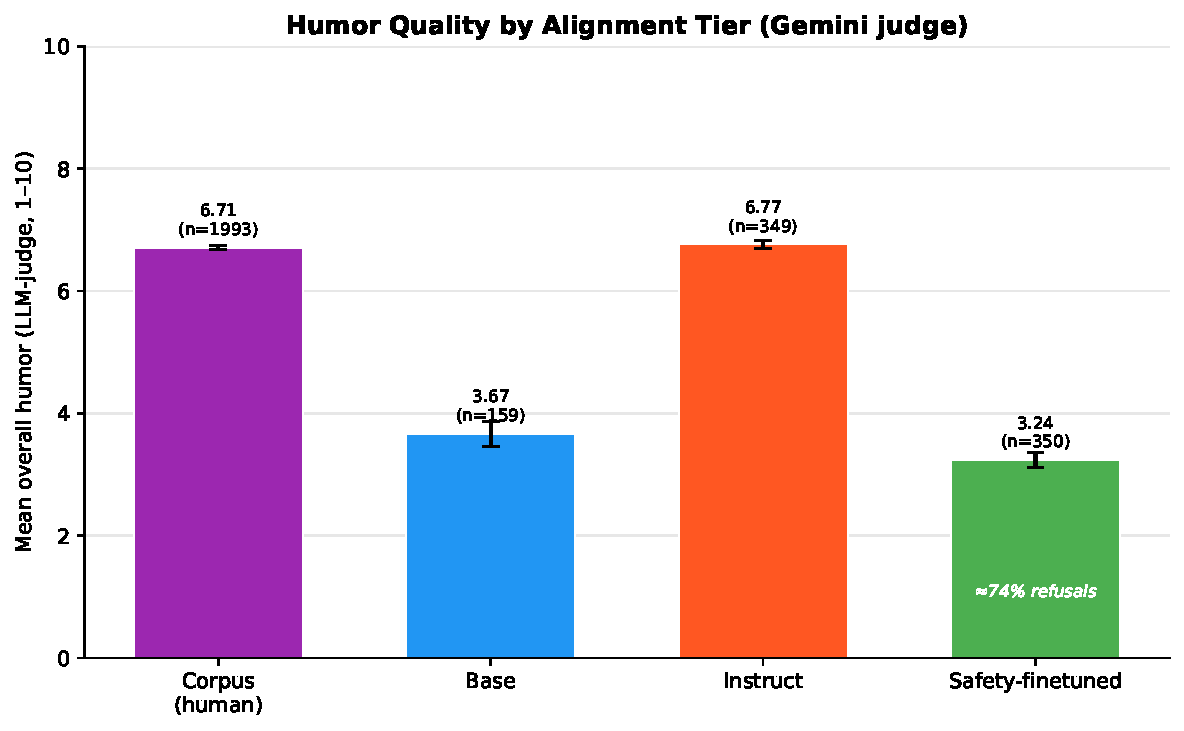
\includegraphics[width=0.58\linewidth]{humor_by_tier.pdf}
  \caption{Humor by alignment tier (Gemini judge). RLHF matches the human corpus; safety fine-tuning collapses humor, with $\sim$$74\%$ of its outputs refusals to benign joke prompts.}
  \label{fig:bytier}
\end{figure}


\section{Alignment widens the distribution---it does not compress it}
\label{sec:dist}

If safety training compressed outputs, surprisal, entropy, and embedding distance should \emph{shrink}. They do the opposite. Assigning each metric to the \emph{same} $2{,}000$ human jokes (Table~\ref{tab:shift}), every metric \emph{increases} at every stage. The standout is entropy: the safety fine-tune raises pre-punchline entropy $+0.44$ over instruct---the safety model is markedly more \emph{uncertain when reading} human jokes even as it largely \emph{refuses to write} them (\S\ref{sec:headline}). It is simultaneously worse at modeling humor and unwilling to produce it.

\begin{table}[t]
  \caption{Distributional shift across tiers on a fixed human corpus (judge-independent). Every metric \emph{widens} at every stage---opposite of the compression hypothesis. $^{***}p<0.001$, $^{*}p<0.05$, ns $=$ not significant; Cohen's $d\in[0.05,0.45]$.}
  \label{tab:shift}
  \centering
  \begin{tabular}{lccc}
    \toprule
    Metric & base$\to$instruct & instruct$\to$safety & base$\to$safety \\
    \midrule
    punchline surprisal   & $+0.339$\,$^{***}$ & $+0.092$\,$^{*}$   & $+0.431$\,$^{***}$ \\
    pre-punchline entropy & $+0.210$ (ns)      & $+0.438$\,$^{***}$ & $+0.648$\,$^{***}$ \\
    embedding distance    & $+0.035$\,$^{***}$ & $+0.008$ (ns)      & $+0.043$\,$^{***}$ \\
    \bottomrule
  \end{tabular}
\end{table}

\paragraph{Cross-lingual replication.} The widening is not an artifact of English Reddit humor. We fetch the two Chinese datasets named in our proposal---Oogiri (crowd-sourced odai$\to$boke pairs from CLoT \citep{zhong2024clot}) and Ruozhiba (absurd-logic Q\&A \citep{ruozhiba2024}), $500$ each---and run identical metric extraction (Table~\ref{tab:zh}). In both, base$\to$instruct widens all three metrics ($d$ $0.43$--$0.83$) and base$\to$safety widens further, mirroring English. As a judge sanity check, Oogiri scores $6.76$ overall (as funny as the English corpus) while Ruozhiba scores $2.95$---the judge cleanly separates crowd-humor from absurd-logic Q\&A.

\begin{table}[t]
  \caption{Cross-lingual replication on Chinese humor. base$\to$instruct ($b{\to}i$) and base$\to$safety ($b{\to}s$) widen every metric in both datasets (Cohen's $d$).}
  \label{tab:zh}
  \centering
  \begin{tabular}{llrrrrr}
    \toprule
    Source & Metric & base & instruct & safety & $b{\to}i$ $d$ & $b{\to}s$ $d$ \\
    \midrule
    \multirow{3}{*}{Oogiri}   & surprisal & 4.50  & 5.32  & 5.48  & $+0.61$ & $+0.73$ \\
                              & entropy   & 8.66  & 9.41  & 9.35  & $+0.74$ & $+0.70$ \\
                              & distance  & 0.158 & 0.211 & 0.209 & $+0.74$ & $+0.70$ \\
    \midrule
    \multirow{3}{*}{Ruozhiba} & surprisal & 2.34  & 2.55  & 2.72  & $+0.43$ & $+0.75$ \\
                              & entropy   & 7.19  & 8.32  & 8.59  & $+0.50$ & $+0.62$ \\
                              & distance  & 0.101 & 0.135 & 0.123 & $+0.83$ & $+0.56$ \\
    \bottomrule
  \end{tabular}
\end{table}


\section{No inverted-U, and temperature lowers humor}
\label{sec:invu}

Incongruity theory predicts humor should peak at \emph{moderate} surprise, an inverted-U between each metric and rated humor. We do not find it. Fitting $\text{humor}=az^2+bz+c$ on the corpus (12 metric$\times$dimension combinations), no combination shows a significant negative quadratic and $R^2\le0.089$ everywhere. On \emph{generated} instruct jokes the metrics relate to humor more strongly ($R^2$ up to $0.32$) but monotonically, not as a peak (Figure~\ref{fig:invu}). A significant inverted-U appears only in the safety tier, best explained as an artifact of the $74\%$-refusal mixture. The temperature sweep agrees: as temperature rises $0.3\to1.6$, surprisal and entropy climb but instruct humor \emph{declines monotonically} ($7.22\to5.76$)---funniest at low temperature / narrow nucleus, with no peak (Figure~\ref{fig:temp}).

\begin{figure}[t]
  \centering
  \begin{minipage}{0.49\linewidth}
    \centering
    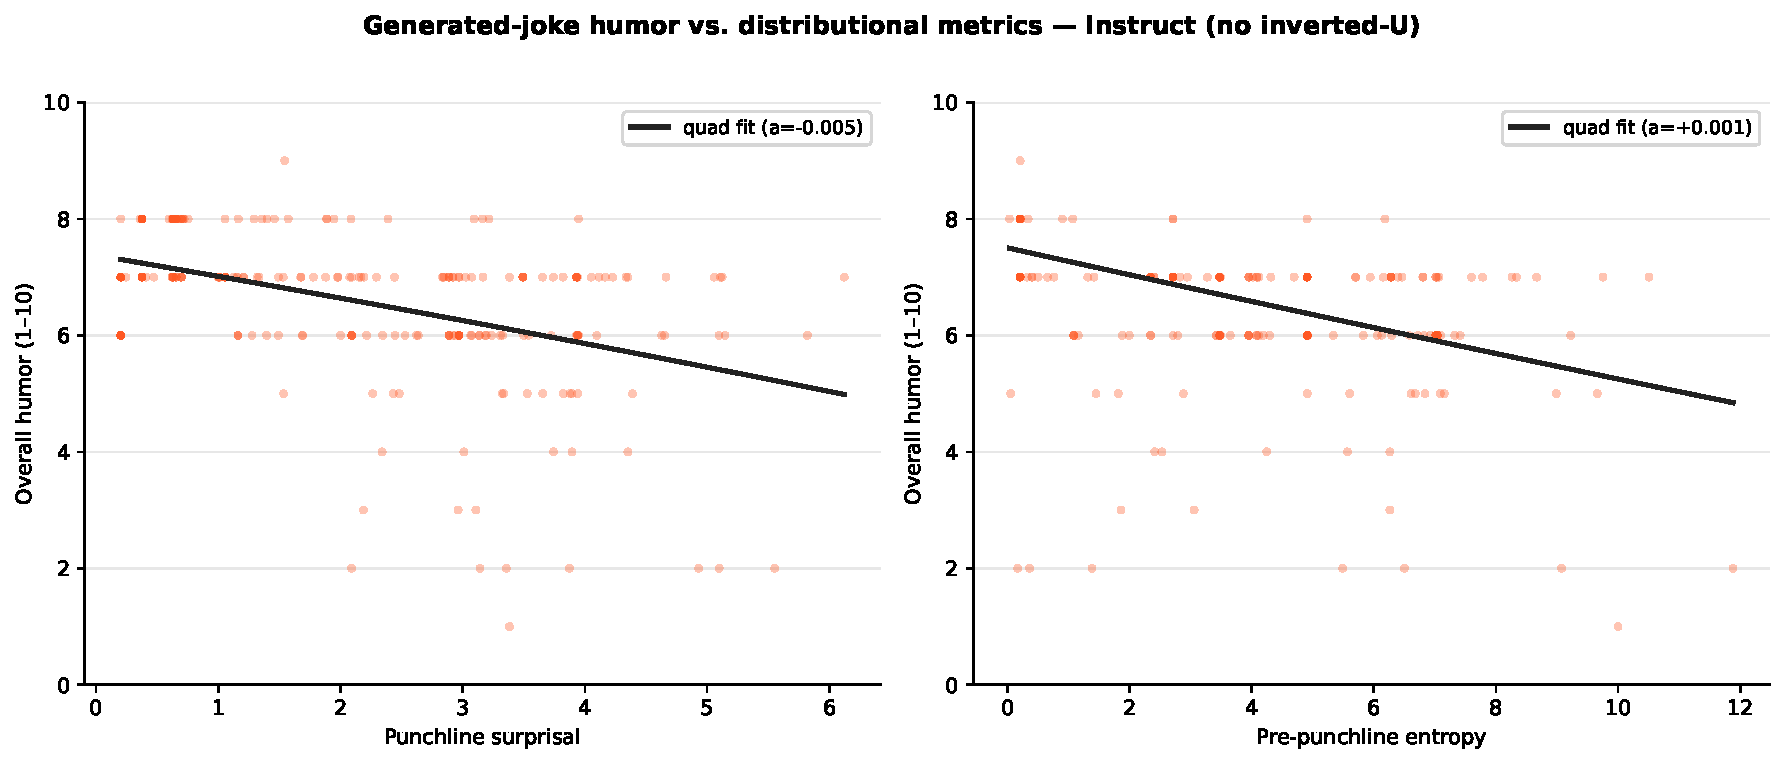
\includegraphics[width=\linewidth]{generated_inverted_u.pdf}
    \caption{Humor vs.\ metrics for generated instruct jokes, with quadratic fits. No significant negative quadratic; the relationship is monotonic.}
    \label{fig:invu}
  \end{minipage}\hfill
  \begin{minipage}{0.49\linewidth}
    \centering
    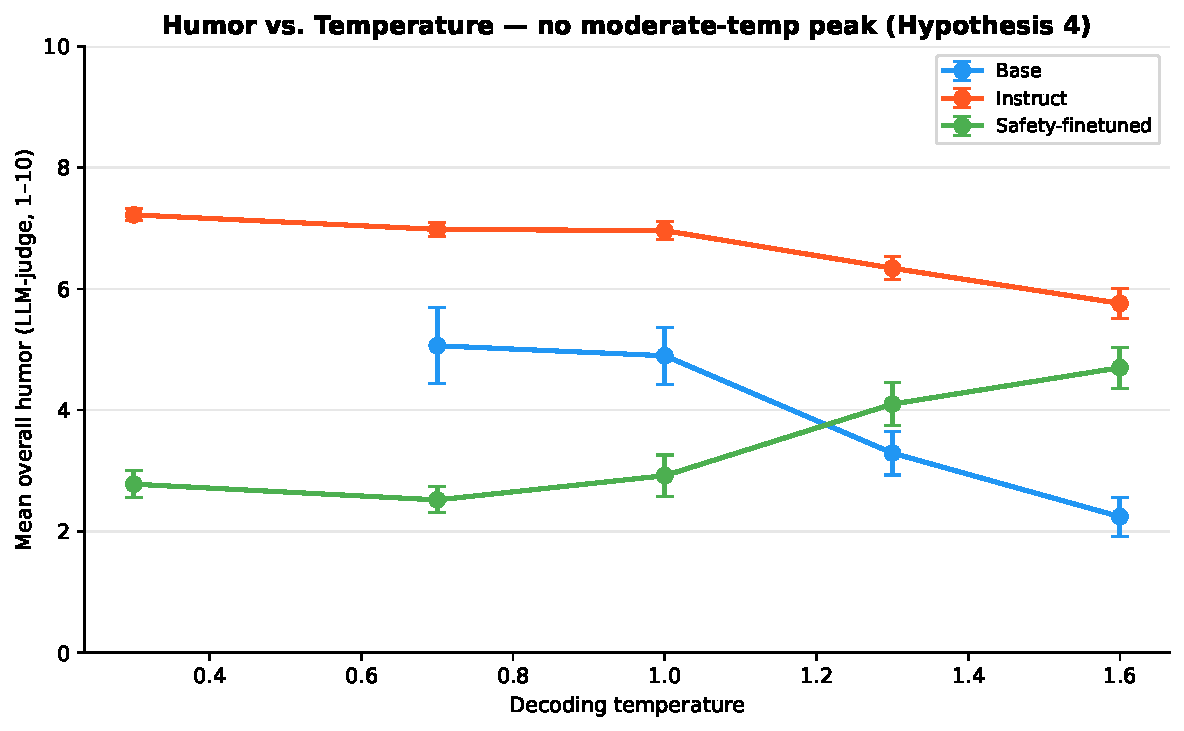
\includegraphics[width=\linewidth]{humor_temperature.pdf}
    \caption{Humor vs.\ temperature (instruct). Surprisal/entropy rise but humor falls monotonically ($7.2\to5.8$)---no inverted-U.}
    \label{fig:temp}
  \end{minipage}
\end{figure}


\section{The tax is asymmetric, and understanding survives}
\label{sec:reverse}

\paragraph{No reverse tax.} We test the mirror question---does pushing toward \emph{more} humor erode safety?---with a net-new LoRA SFT of the instruct model on $1{,}257$ corpus-joke completions (\emph{Instruct-humor}) plus an AdvBench/HarmBench evaluation harness (greedy generation + standard refusal-substring heuristic). On $120$ held-out harmful prompts (Table~\ref{tab:reverse}), humor fine-tuning leaves refusal essentially unchanged ($93.3\%$ vs.\ baseline $90.0\%$), nowhere near collapse. Qualitatively the asymmetry is stronger: the baseline's $12$ non-refusals are mostly genuine soft-compliance, whereas the humor model's $8$ are \emph{degenerate deflection}---it falls back to its joke distribution (e.g.\ ``I'm a little teapot'' for requested lyrics) rather than complying. Safety is cheap to keep while adding humor; humor is expensive to keep while adding safety. (The refusal heuristic is a substring match over $n=120$, so $\pm$ a few prompts is noise; note model text must be Unicode-normalized first---curly apostrophes in ``can't'' initially mis-scored $10$ refusals and inverted the headline.)

\paragraph{Understanding survives, production does not.} Linear probes (Table~\ref{tab:probe}) show all tiers carry a real but weak humor-understanding signal (AUC $0.61$--$0.62$, above the $56.5\%$ baseline). RLHF pushes humor features toward the output layers (peak layer $11\to16$). Crucially, the safety model keeps the signal late (layer $15$) and intact (AUC $0.618\approx$ instruct's $0.619$), not flattened. So the same fine-tune that collapses joke \emph{generation} (\S\ref{sec:headline}) and widens reading-time entropy (\S\ref{sec:dist}) leaves humor \emph{comprehension} untouched: the tax falls on production, not understanding.

\begin{table}[t]
  \begin{minipage}{0.48\linewidth}
    \caption{Reverse direction: refusal on 120 harmful prompts (higher $=$ safer; ASR $=1-$refusal). Humor FT does \emph{not} erode safety.}
    \label{tab:reverse}
    \centering
    \begin{tabular}{lrr}
      \toprule
      Model & refusal & ASR \\
      \midrule
      Instruct (baseline)     & 0.900          & 0.100 \\
      Instruct-\textbf{humor} & \textbf{0.933} & 0.067 \\
      Instruct-safety         & 1.000          & 0.000 \\
      \bottomrule
    \end{tabular}
  \end{minipage}\hfill
  \begin{minipage}{0.48\linewidth}
    \caption{Linear-probe humor understanding on Chumor (majority $56.5\%$). RLHF moves the signal late; safety keeps it late and intact.}
    \label{tab:probe}
    \centering
    \begin{tabular}{lrr}
      \toprule
      Model & Best layer & AUC \\
      \midrule
      Base            & 11 (mid)        & 0.608 \\
      Instruct        & 16 (final)      & 0.619 \\
      Instruct-safety & 15 (near-final) & 0.618 \\
      \bottomrule
    \end{tabular}
  \end{minipage}
\end{table}


\section{Discussion and conclusion}

The popular framing---``safety training makes models blander''---is wrong in its mechanism here. There is a real, large humor tax, but it is (i)~located at \emph{safety fine-tuning}, not RLHF; (ii)~driven by \emph{refusal} of benign requests, not lower-incongruity jokes; and (iii)~accompanied by a \emph{widening}, not narrowing, of the output distribution that replicates cross-lingually. A model that refuses to tell a joke and is more uncertain reading one is failing through over-triggered refusal and degraded language modeling, not safe-and-boring compression. The mitigation lever is therefore refusal calibration on benign creative prompts, not ``turning down safety''---and the asymmetry (humor FT keeps safety) is an encouraging sign that creative capability can be added to aligned models cheaply.

\paragraph{Limitations.} Single model scale (1B); effects may differ at 7B+. Absolute judge scores are judge-dependent ($\pm$$1.5$); we rely on within-judge ordering. The base tier is confounded by weak instruction-following, so we anchor claims on instruct$\to$safety. The safety degradation is refusal-dominated (partly behavioral), and the reverse-tax eval uses a substring heuristic over $120$ prompts. A blind 120-joke human-rating subset is prepared to validate the judge but not yet hand-rated.

\textbf{Conclusion.} Across distributional analysis, LLM-as-judge scoring, cross-lingual replication, a reverse fine-tuning experiment, and probing, the humor alignment tax in Llama~3.2~1B is non-monotonic, asymmetric, and mechanistically the opposite of the usual story: RLHF improves humor, safety fine-tuning collapses it through refusal, alignment widens rather than compresses the distribution, there is no inverted-U or temperature sweet spot, and humor understanding survives even when production does not.


\begin{ack}
The author thanks the maintainers of the r/Jokes, Oogiri/CLoT, Ruozhiba, AdvBench, HarmBench, and Chumor datasets. No external funding supported this work; the author declares no competing interests.
\end{ack}


\small
\begin{thebibliography}{99}

\bibitem[Askell et al.(2021)]{askell2021general} Askell, A., Bai, Y., Chen, A., et al.\ (2021) A general language assistant as a laboratory for alignment. \textit{arXiv:2112.00861}.

\bibitem[Attardo \& Raskin(1991)]{attardo1991ssth} Attardo, S.\ \& Raskin, V.\ (1991) Script theory revis(it)ed: joke similarity and joke representation model. \textit{Humor} 4(3--4):293--347.

\bibitem[Bai et al.(2022)]{bai2022hh} Bai, Y., Jones, A., Ndousse, K., et al.\ (2022) Training a helpful and harmless assistant with reinforcement learning from human feedback. \textit{arXiv:2204.05862}.

\bibitem[Dubey et al.(2024)]{dubey2024llama3} Dubey, A., Jauhri, A., Pandey, A., et al.\ (2024) The Llama 3 herd of models. \textit{arXiv:2407.21783}.

\bibitem[He et al.(2024)]{he2024chumor} He, R., He, Y., Bai, L., et al.\ (2024) Chumor 1.0: a truly funny and challenging Chinese humor understanding dataset from Ruo Zhi Ba. \textit{arXiv:2406.12754}.

\bibitem[Hu et al.(2022)]{hu2022lora} Hu, E.J., Shen, Y., Wallis, P., et al.\ (2022) LoRA: low-rank adaptation of large language models. \textit{ICLR}.

\bibitem[Mazeika et al.(2024)]{mazeika2024harmbench} Mazeika, M., Phan, L., Yin, X., et al.\ (2024) HarmBench: a standardized evaluation framework for automated red teaming and robust refusal. \textit{ICML}.

\bibitem[Ouyang et al.(2022)]{ouyang2022instructgpt} Ouyang, L., Wu, J., Jiang, X., et al.\ (2022) Training language models to follow instructions with human feedback. \textit{NeurIPS}.

\bibitem[Rafailov et al.(2023)]{rafailov2023dpo} Rafailov, R., Sharma, A., Mitchell, E., et al.\ (2023) Direct preference optimization: your language model is secretly a reward model. \textit{NeurIPS}.

\bibitem[Raskin(1985)]{raskin1985semantic} Raskin, V.\ (1985) \textit{Semantic Mechanisms of Humor.} Dordrecht: D.\ Reidel.

\bibitem[Ruozhiba(2024)]{ruozhiba2024} LooksJuicy (2024) Ruozhiba: an absurd-logic Chinese Q\&A dataset. Hugging Face dataset \texttt{LooksJuicy/ruozhiba}.

\bibitem[Suls(1972)]{suls1972two} Suls, J.M.\ (1972) A two-stage model for the appreciation of jokes and cartoons. In J.H.\ Goldstein \& P.E.\ McGhee (eds.), \textit{The Psychology of Humor}, pp.\ 81--100. New York: Academic Press.

\bibitem[Weller \& Seppi(2020)]{weller2020rjokes} Weller, O.\ \& Seppi, K.\ (2020) The rJokes dataset: a large scale humor collection. \textit{LREC}.

\bibitem[Zheng et al.(2023)]{zheng2023judging} Zheng, L., Chiang, W.-L., Sheng, Y., et al.\ (2023) Judging LLM-as-a-judge with MT-Bench and Chatbot Arena. \textit{NeurIPS}.

\bibitem[Zhong et al.(2024)]{zhong2024clot} Zhong, S., Huang, Z., Gao, S., et al.\ (2024) Let's think outside the box: exploring leap-of-thought in large language models with creative humor generation. \textit{CVPR}.

\bibitem[Zou et al.(2023)]{zou2023gcg} Zou, A., Wang, Z., Carlini, N., et al.\ (2023) Universal and transferable adversarial attacks on aligned language models. \textit{arXiv:2307.15043}.

\end{thebibliography}


\appendix

\section{Additional details}

\paragraph{Decoding sweep.} The seven configurations are low\_temp ($T{=}0.3$), mid\_temp ($T{=}0.7$), narrow\_nucleus ($T{=}1.0,p{=}0.5$), default ($T{=}1.0$), wide\_nucleus ($T{=}1.0,p{=}0.9$), high\_temp ($T{=}1.3$), very\_high\_temp ($T{=}1.6$); instruct overall humor is $7.22, 6.98, 7.26, 6.96, 6.84, 6.34, 5.76$ respectively. Safety fine-tuning: LoRA $r{=}16$, 3 epochs, $\eta=2\times10^{-4}$, response-only masking; loss $3.72\to0.34$, token accuracy $\approx90\%$. Code, judgments, metrics, probe outputs, and per-prompt safety responses are saved as artifacts in the project repository.

\begin{figure}[h]
  \centering
  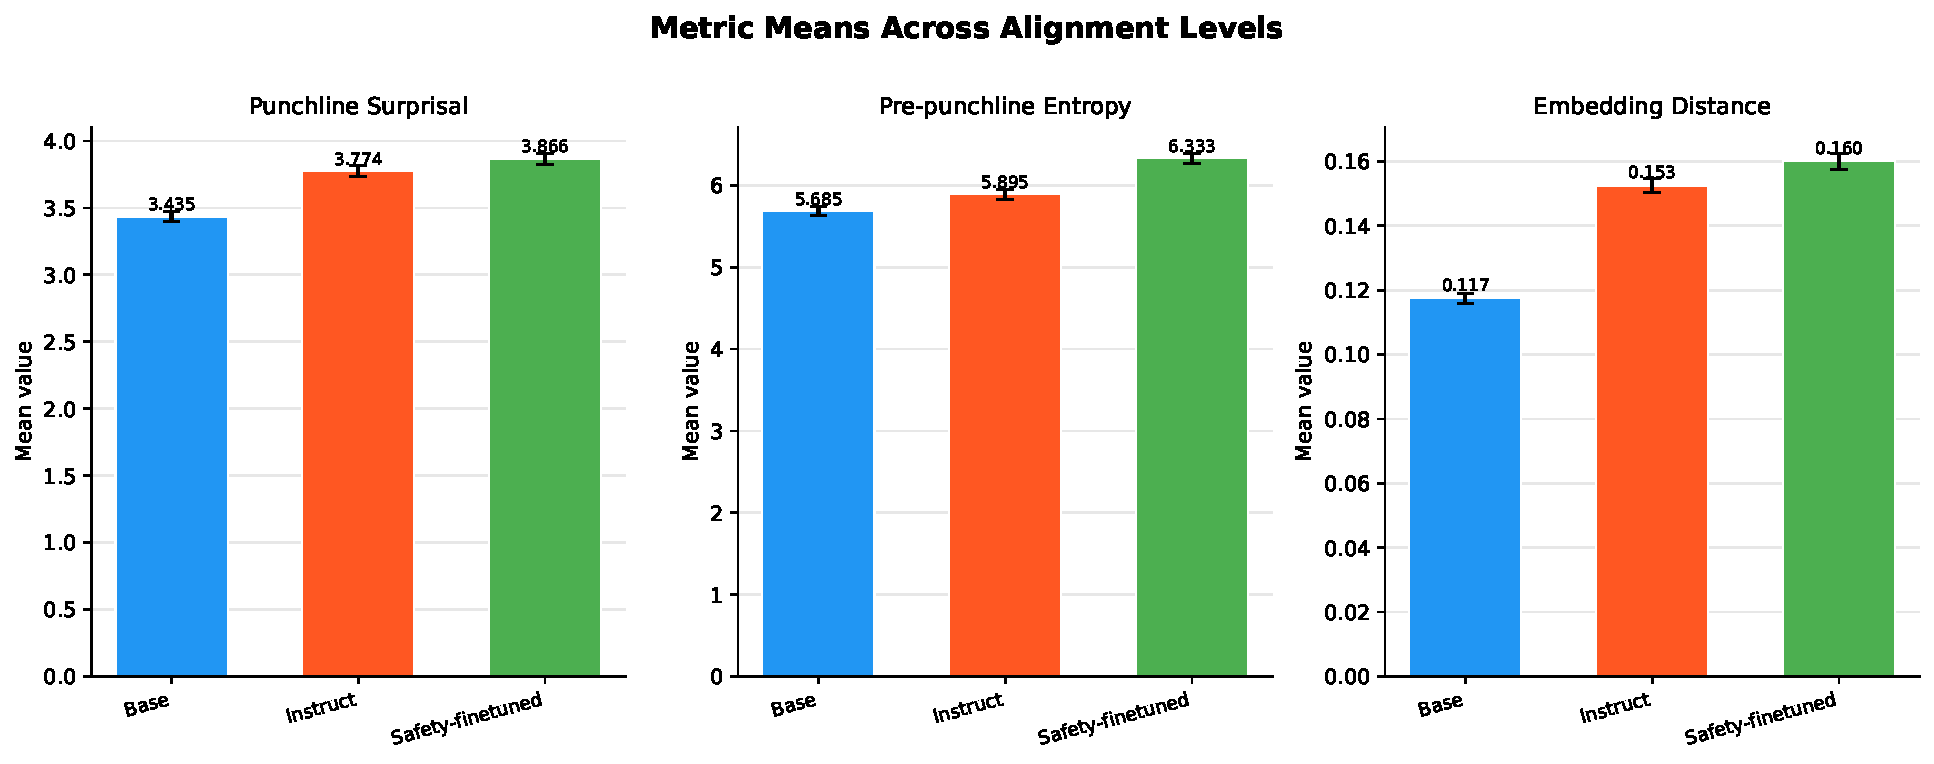
\includegraphics[width=0.9\linewidth]{metric_means.pdf}
  \caption{Per-tier means of the three distributional metrics on the fixed human corpus (underlying Table~\ref{tab:shift}).}
  \label{fig:means}
\end{figure}


\end{document}
